% \documentclass[../ThesisDoc]{subfiles}
\documentclass{standalone}

\usepackage{tikz, pgfplots}
\usetikzlibrary{fit, matrix, positioning, shapes, decorations.pathreplacing,
                shapes.geometric, chains, arrows, calc }



\newcommand{\mkInnerSide}[4][]{
  \shade[top color=gray!10, bottom color=black!50, #1] (0,0) rectangle +(5,5);
  % grid
  \draw (0,0) grid (5,5);
  % header
  \foreach \i/\x in {1/#2_1,2/\dots,3/#2_#3,4/\dots,5/#2_#4}
    { \node (#2-header-\i) at (\i-0.5, 4.5) {$\x$}; }
  % center
  \node[inner sep=0pt] (#2-center) at (2.5,2.5) {};
  % corners
  \node[inner sep=0pt] (#2-bottom-left)  at (0,0) {};
  \node[inner sep=0pt] (#2-bottom-right) at (5,0) {};
  \node[inner sep=0pt] (#2-top-right)    at (5,5) {};
  \node[inner sep=0pt] (#2-top-left)     at (0,5) {};
}


\newcommand{\mkOuterSide}[3]{
  \draw[#1] (-5,-5) rectangle (10,10);
  \draw[#2] (#3-bottom-left)  -- (-5,-5);
  \draw[#2] (#3-bottom-right) -- (10,-5);
  \draw[#2] (#3-top-right)    -- (10,10);
  \draw[#2] (#3-top-left)     -- (-5,10);
}


%from http://www.texample.net/tikz/examples/sudoku-3d-cube/
\begin{document}


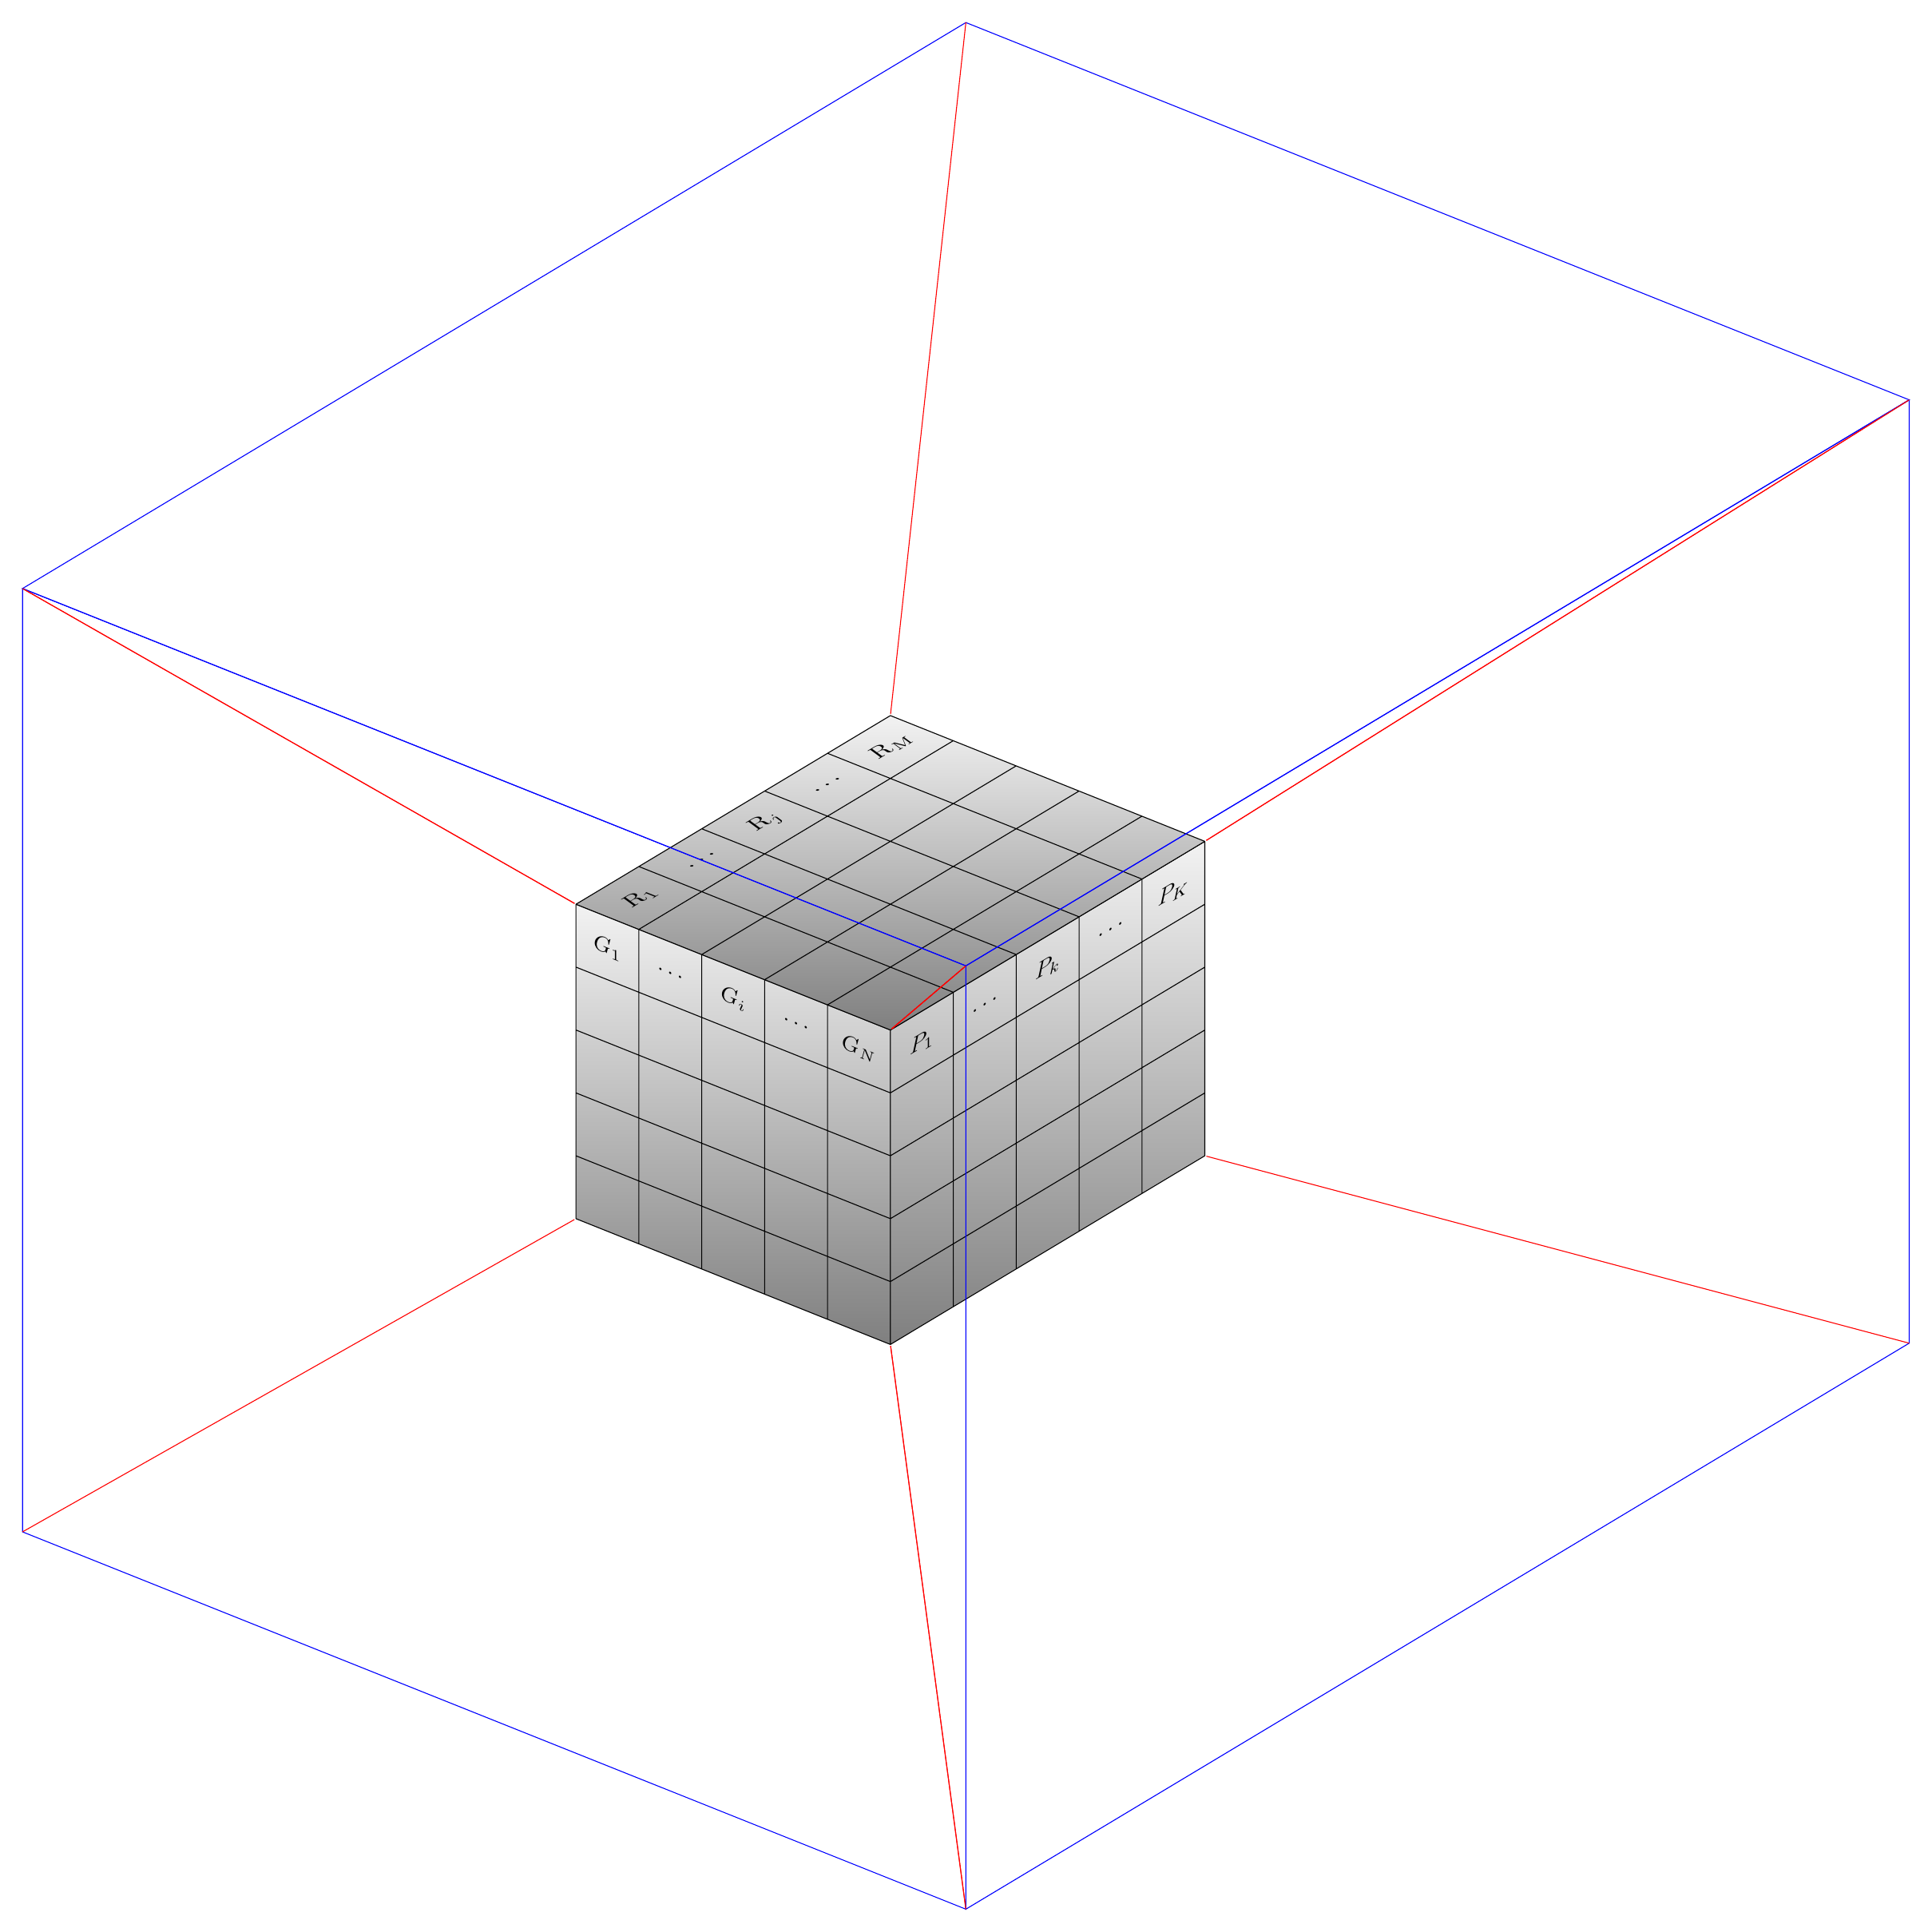
\begin{tikzpicture}[
  sideXS/.style={yslant=-0.4},
  sideYS/.style={yslant=0.6},
  sideZS/.style={yslant=0.6,xslant=-1},
  sideX/.style={every node/.append style={sideXS}, sideXS},
  sideY/.style={every node/.append style={sideYS}, sideYS},
  sideZ/.style={every node/.append style={sideZS}, sideZS},
  ]


\begin{scope}[sideX]
  \mkInnerSide{G}{i}{N}
\end{scope}
\begin{scope}[xshift=5cm, yshift=-2cm, sideY]
  \mkInnerSide{P}{k}{K}
\end{scope}
\begin{scope}[xshift=5cm, yshift=3cm, sideZ]
  \mkInnerSide{R}{j}{M}
\end{scope}

\begin{scope}[xshift=-5cm, sideX, yshift=-1.5cm, xshift=1.2cm]
  \mkOuterSide{blue}{red}{G}
\end{scope}
\begin{scope}[xshift=5cm, yshift=-6.7cm, sideY, xshift=6.2cm]
  \mkOuterSide{blue}{red}{P}
\end{scope}
\begin{scope}[xshift=5cm, yshift=8.3cm, sideZ, xshift=1.2cm]
  \mkOuterSide{blue}{red}{R}
\end{scope}

\end{tikzpicture}
\end{document}
